%%
%% Copyright 2007, 2008, 2009 Elsevier Ltd
%%
%% This file is part of the 'Elsarticle Bundle'.
%% ---------------------------------------------
%%
%% It may be distributed under the conditions of the LaTeX Project Public
%% License, either version 1.2 of this license or (at your option) any
%% later version.  The latest version of this license is in
%%    http://www.latex-project.org/lppl.txt
%% and version 1.2 or later is part of all distributions of LaTeX
%% version 1999/12/01 or later.
%%
%% This template has been modified by Philip Blakely for
%% local distribution to students on the MPhil for Scientific
%% Computing course run at the University of Cambridge.
%%

%% Template article for Elsevier's document class `elsarticle'
%% with numbered style bibliographic references
%% SP 2008/03/01
%%
%%
%%
%% $Id: elsarticle-template-num.tex 4 2009-10-24 08:22:58Z rishi $

\documentclass[final,3p,times,twocolumn]{elsarticle}
\usepackage{pdfpages}
\usepackage{booktabs} % Tables
\usepackage{pifont}

%% Use the option review to obtain double line spacing
%% \documentclass[preprint,review,12pt]{elsarticle}

%% Use the options 1p,twocolumn; 3p; 3p,twocolumn; 5p; or 5p,twocolumn
%% for a journal layout:
%% \documentclass[final,1p,times]{elsarticle}
%% \documentclass[final,1p,times,twocolumn]{elsarticle}
%% \documentclass[final,3p,times]{elsarticle}
%% \documentclass[final,3p,times,twocolumn]{elsarticle}
%% \documentclass[final,5p,times]{elsarticle}
%% \documentclass[final,5p,times,twocolumn]{elsarticle}

%% if you use PostScript figures in your article
%% use the graphics package for simple commands
%% \usepackage{graphics}
%% or use the graphicx package for more complicated commands
%% \usepackage{graphicx}
%% or use the epsfig package if you prefer to use the old commands
%% \usepackage{epsfig}

%% The amssymb package provides various useful mathematical symbols
\usepackage{amssymb}
\usepackage{float}
\usepackage{subfig}
\usepackage{graphicx}
\usepackage{soul}

%% Font setting, for my own eyes
\usepackage{libertine}
\usepackage{libertinust1math}
\usepackage[T1]{fontenc}

%% Algorithms
\usepackage[ruled,vlined]{algorithm2e}

%% Some math characters
\usepackage{bbold}


%% So that references are listed in the Contents
\usepackage[nottoc,notlot,notlof]{tocbibind}

\newcommand{\cmark}{\ding{51}}%
\newcommand{\xmark}{\ding{55}}%

%% The amsthm package provides extended theorem environments
%% \usepackage{amsthm}

%% The lineno packages adds line numbers. Start line numbering with
%% \begin{linenumbers}, end it with \end{linenumbers}. Or switch it on
%% for the whole article with \linenumbers after \end{frontmatter}.
%% \usepackage{lineno}

%% natbib.sty is loaded by default. However, natbib options can be
%% provided with \biboptions{...} command. Following options are
%% valid:

%%   round  -  round parentheses are used (default)
%%   square -  square brackets are used   [option]
%%   curly  -  curly braces are used      {option}
%%   angle  -  angle brackets are used    <option>
%%   semicolon  -  multiple citations separated by semi-colon
%%   colon  - same as semicolon, an earlier confusion
%%   comma  -  separated by comma
%%   numbers-  selects numerical citations
%%   super  -  numerical citations as superscripts
%%   sort   -  sorts multiple citations according to order in ref. list
%%   sort&compress   -  like sort, but also compresses numerical citations
%%   compress - compresses without sorting
%%
%% \biboptions{comma,round}

% \biboptions{}


\journal{MPhil in Scientific Computing}
%\setlength{\columnseprule}{0.2pt}

\begin{document}

\begin{frontmatter}

%% Title, authors and addresses

%% use the tnoteref command within \title for footnotes;
%% use the tnotetext command for the associated footnote;
%% use the fnref command within \author or \address for footnotes;
%% use the fntext command for the associated footnote;
%% use the corref command within \author for corresponding author footnotes;
%% use the cortext command for the associated footnote;
%% use the ead command for the email address,
%% and the form \ead[url] for the home page:
%%
%% \title{Title\tnoteref{label1}}
%% \tnotetext[label1]{}
%% \author{Name\corref{cor1}\fnref{label2}}
%% \ead{email address}
%% \ead[url]{home page}
%% \fntext[label2]{}
%% \cortext[cor1]{}
%% \address{Address\fnref{label3}}
%% \fntext[label3]{}

\title{Variational Autoencoders with variance loss}

%% use optional labels to link authors explicitly to addresses:
%% \author[label1,label2]{<author name>}
%% \address[label1]{<address>}
%% \address[label2]{<address>}

\author{Bla\v z Stojanovi\v c}

\address{Cavendish Laboratory, Department of Physics, J J Thomson
  Avenue, Cambridge. CB3 0HE}

\begin{abstract}

\end{abstract}

\end{frontmatter}

%%
%% Start line numbering here if you want
%%
% \linenumbers

%% main text
\tableofcontents
\section{Introduction}
\subsection{Generative modelling}
Depending on what we learn in machine learning we differentiate between \emph{discriminative} and \emph{generative} modelling. While there is some inconsistency in the terminology, at their core discriminative models only have the ability to discriminate between targets $Y$ and inputs $X$ while generative models "simulate" the underlying data generation process and have the ability to generate new samples from the underlying distribution of data. Generative modelling is very much similar to the scientific process of providing competing models of how physical phenomena work and testing them through observations. The models are considered highly intuitive and interpretable as we can encode our prior knowledge into them while treating unknown details as noise~\cite{kingma2017variational}. While there has been a recent surge of popularity in generative modeling, with models like the \emph{variational autoencoder} (VAE)~\cite{kingma2013auto, rezende2014stochastic}, \emph{Generative Adversarial Network} (GAN)~\cite{goodfellow2016nips} and \emph{Normalizing Flows}~\cite{rezende2015variational} generative modelling in ML has a rich history. Models such as Gaussian mixture models~\cite{everitt2014finite}, Hidden Markov models~\cite{rabiner1986introduction}, Autoregressive models, Latent Dirichlet allocation~\cite{blei2003latent}, Boltzmann and Helmholtz machines~\cite{ackley1985learning, dayan1995helmholtz} have long been known and used. With increase in computational power, modern generative models have achieved astounding results in speech synthesis~\cite{oord2016wavenet}, image super-resolution~\cite{ledig2017photo} and have been implemented to aid supervised learning~\cite{kingma2014semi}. 

Ian Goodfellow provided a helpful taxonomy of generative models in his tutorial on GANs~\cite{goodfellow2016nips}. He differentiates generative models that maximise likelihood between how they compute or approximate the likelihood and its gradients. The model can construct an explicit probability density $p_{\boldsymbol{\theta}}(\mathbf{x})$ and consequently an explicit likelihood which is then optimised. This explicit density can either be tractable as is the case in \emph{fully observed Bayesian networks}, or it could be intractable requiring either variational approaches as in the VAE, or MCMC for example in Boltzmann machines. On the other hand we have models that do not construct the probability distribution explicitly, but instead provide a less direct way to interact with it i.e. draw samples from it. GANs fall into this category. 

\subsection{Deep latent variable models}
\label{sec:DLVM}
We assume that an observable value $\mathbf{x}$ is generated by an unknown underlying random process with unknown probability distribution $p^*(\mathbf{x})$. This is the process we try to approximate using a generative model $p_{\boldsymbol{\theta}}(\mathbf{x})$, which is parameterised with parameters $\boldsymbol{\theta}$. The process of learning is finding parameters $\boldsymbol{\theta}$ such that our model distribution $p_{\boldsymbol{\theta}}(\mathbf{x})$ is as close to the underlying distribution $p^*(\mathbf{x})$. Normally though, this is the case for regression and classification problems, we are modelling the conditional distribution $p^{*}(\mathbf{y} | \mathbf{x})$ with our model $p_{\boldsymbol{\theta}}(\mathbf{y} | \mathbf{x})$, where $\mathbf{y}$ is conditioned on the input $\mathbf{x}$. The approaches described and implemented in this written assignment are equally applicable to both conditional and unconditional modelling. In either case we want our model to be versatile enough to represent the underlying structure of the data. The last two decades have seen a renaissance of neural networks as models of complex processes~\cite{goodfellow2016deep}, they are \emph{universal function approximators}, generally made of compositions of smaller differentiable sub-units with nonlinear activation functions and trained using gradient-based approaches via backpropagation. They can be used to parameterize conditional distributions and form basis of probabilistic models thus combining the best of both worlds, a probabilistic description and \emph{hopefully} better scalability, making use of gradient-based learning. The categorical distribution $p_{\boldsymbol{\theta}}(y|\mathbf{x})$ in the case of classification, where $y$ is the class, given the input $\mathbf{x}$, can be parameterised as
\begin{equation}
	\begin{aligned}
			\mathbf{p} &= f(\mathbf{x}; \boldsymbol{\theta}), \\
			p_{\boldsymbol{\theta}}(y | \mathbf{x})&=\operatorname{Categorical}(y ; \mathbf{p}),
	\end{aligned}
\end{equation}
where $f(\cdot, \boldsymbol{\theta}): \mathbb{R}^{n_{\mathrm{in}}} \rightarrow \mathbb{R}^{n_{\mathrm{out}}}$ is the neural network, with a final layer such that the probabilities $\sum_{i}^{n_\mathrm{out}} p_{i}=~1$. 

We can combine random variables $(\mathbf{x_1}, \ldots, \mathbf{x_M})$ and represent their conditional dependence structure as a network to construct a \emph{probabilistic graphical model}. If the structure of the network is a directed acyclic graph, the joint distribution of the random variables is factorised as a product of conditionals and priors
\begin{equation}
	p_{\boldsymbol{\theta}}\left(\mathbf{x}_{1}, \ldots, \mathbf{x}_{M}\right)=\prod_{j=1}^{M} p_{\boldsymbol{\theta}}\left(\mathbf{x}_{j} \mid \mathrm{pa}(\mathbf{x}_{j})\right),
\end{equation}
where $ \mathrm{pa}(\mathbf{x}_{j})$ are the parent nodes of node $j$ in the directed graph. A graphical model with this structure is termed a \emph{Bayesian network} and we can parameterise the conditional distributions in a Bayesian network using neural networks
\begin{equation}
	\begin{aligned} 
		\boldsymbol{\eta} &=f(\mathrm{pa}(\mathbf{x}); \boldsymbol{\theta}) \\ p_{\boldsymbol{\theta}}(\mathbf{x} \mid \mathrm{pa}(\mathbf{x})) &=p_{\boldsymbol{\theta}}(\mathbf{x} \mid \boldsymbol{\eta}). 
	\end{aligned}
\end{equation}
A model which only contains observable variables $\mathbf{x}_i$ is a \emph{fully observed} model and is straightforward to learn. Given a dataset $\mathcal D$ of \emph{independently and identically distributed} observations $\mathbf{x}_i$ we can perform \emph{maximum likelihood estimation}, i.e. search for parameters $\boldsymbol{\theta}$ such that the observed data is most probable, by simply estimating the gradients of the \emph{log-likelihood}
\begin{equation}
	\log p_{\theta}(\mathcal{D})=\sum_{\mathbf{x} \in \mathcal{D}} \log p_{\theta}(\mathbf{x})
\end{equation}
Moreover, \emph{maximum a posteriori estimation} of which maximum likelihood is a special case, can be performed and full Bayesian treatment of the posterior is also possible~\cite{kingma2017variational}. 
A complication arises when we include \emph{latent} variables into the model, these are variables which are not observable and do not form a part of the dataset $\mathcal D$, usually denoted with $\mathbf{z}$. For unconditional model learning the graphical model now represents a joint probability distribution $p_{\boldsymbol{\theta}}(\mathbf{x}, \mathbf{z})$, which when marginalized gives the single point \emph{model evidence} $p_{\boldsymbol{\theta}}(\mathbf{x})$ as a function of the parameters $\boldsymbol{\theta}$. In the simplest deep latent variable models, the joint probability is factored into the prior distribution $p_{\theta}(\mathbf{z})$ and the conditional distribution, which is represented by a neural network $p_{\boldsymbol{\theta}}(\mathbf{x}|\mathbf{z})$,  as
\begin{equation}
	p_{\boldsymbol{\theta}}(\mathbf{x}, \mathbf{z})=p_{\boldsymbol{\theta}}(\mathbf{z}) p_{\boldsymbol{\theta}}(\mathbf{x} \mid \mathbf{z}).
\end{equation}
Alternatively, we can have a model with many layers of latent variables $\mathbf{z}_m$,
\begin{equation}
	p_{\boldsymbol{\theta}}(\mathbf{x}, \mathbf{\mathbf{z}}) = p\left(x \mid \mathbf{z}_{1}\right) p\left(\mathbf{z}_{1} \mid \mathbf{z}_{2}\right) \cdots p\left(\mathbf{z}_{m-1} \mid \mathbf{z}_{m}\right) p\left(\mathbf{z}_{m}\right),
\end{equation} 
which are then able to learn hierarchical latent representation. In either case learning the posterior $p_{\theta}(\mathbf{x}, \mathbf{z})$, i.e.
\begin{equation}
	p_{\boldsymbol{\theta}}(\mathbf{x})=\int p_{\boldsymbol{\theta}}(\mathbf{x}, \mathbf{z}) d \mathbf{z},
\end{equation}
is intractable, meaning it is (without tricks) impossible to differentiate the marginal likelihood w.r.t parameters $\boldsymbol{\theta}$ and perform gradient-based optimisation. Advantage of DLVMs is their flexibility, even using very simple priors and conditionals they can express complicated distributions because of the nonlinearity of the neural network representations. 

\subsubsection{Learning in DLVMs}
There are two main issues with learning in deep latent variable models, succinctly illustrated with two optimisation approaches. The first is the Expectation-Maximization (EM)~\cite{dempster1977maximum} algorithm, it consists of two steps which are repeated until convergence.
\begin{itemize}
	\item \textbf{E-step}: For each datapoint $\mathbf{x}_i$ compute the posterior $p_{\boldsymbol{\theta}_t}(\mathbf{z}_i|\mathbf{x_i})$.
	\item \textbf{M-step}: Estimate new parameters by maximsing the expected log-likelihood $\theta_{t+1}=\arg \max _{\theta} \sum_{x \in D} \mathbb{E}_{z \sim p\left(z | x ; \theta_{t}\right)} \log p(x, z ; \theta)$.
\end{itemize}
The algorithm falls apart in two ways, firstly the E-step requires computation of the posterior distribution which is intractable in DLVMs. This can be solved by employing a sampling technique (MCMC EM algorithm) but at a high computational cost, requiring a per datapoint MCMC step. Secondly, the M-step optimises over all datapoints requiring vast amounts of memory, although it can be done in mini-batches (online EM~\cite{hoffman2010online}. Hence, the first issue with learning in DLVMs is computational efficiency. The second algorithm is the \emph{wake-sleep} algorithm~\cite{hinton1995wake}, it employs a recognition model that approximates the posterior distribution and is applicable to both discrete and continuous latent variable models. While it is not computationally expensive relative to EM, its optimisation objectives do not coincide with optimising the marginal likelihood, thus giving a bad estimate of the posterior. Therefore the second issue is inaccurate estimates of the posterior. Both these issues were addressed in two seminal papers that constitute the framework of the variational autoencoder~\cite{kingma2013auto, rezende2014stochastic}. 

\subsection{Variational Autoencoders}
\label{sec:ELBO}
The strength of variational methods lies in recasting inference as an optimisation problem, which scales better to large datasets than sampling methods. This is done by introducing an approximate posterior distribution $q_{\boldsymbol{\phi}}(\mathbf{z} | \mathbf{x})$, with parameters $\boldsymbol{\phi}$ and optimising to maximise the similarity between $q_{\boldsymbol{\phi}}(\mathbf{z} | \mathbf{x})$ and $p_{\boldsymbol{\theta}}(\mathbf{z} | \mathbf{x})$. In the case of the VAE $q_{\boldsymbol{\phi}}(\mathbf{z} | \mathbf{x})$ is also parameterised using a neural network. The similarity between the two distributions is measured by the Kullback-Leibler divergence 
\begin{equation}
	D_{KL}(q \| p)=\sum_{\mathbf{x}} q(\mathbf{x}) \log \frac{q(\mathbf{x})}{p(\mathbf{x})},
\end{equation}
which has two important properties $D_{KL}(q \| p) \geq 0$ for all $q$ and $p$ and it is equal to zero only when $q = p$. It can be rewritten as
\begin{equation}
	\begin{aligned}
		&D_{K L}(q_{\boldsymbol{\phi}}(\mathbf{z} \mid \mathbf{x}) \| p_{\boldsymbol{\theta}}(\mathbf{z} \mid \mathbf{x})) = \\ 
		&= \sum_{\mathbf{z}} q_{\boldsymbol{\phi}}(\mathbf{z} | \mathbf{x})\left[\log \frac{q_{\boldsymbol{\phi}}(\mathbf{z} | \mathbf{x})}{p_{\boldsymbol{\theta}}(\mathbf{z}, \mathbf{x})}+\log p_{\boldsymbol{\theta}}(\mathbf{x})\right]  \\
		&= \sum_{\mathbf{z}} q_{\boldsymbol{\phi}}(\mathbf{z} | \mathbf{x})\left[\log q_{\boldsymbol{\phi}}(\mathbf{z} | \mathbf{x}) - \log p_{\boldsymbol{\theta}}(\mathbf{z}, \mathbf{x}) \right] + q_{\boldsymbol{\phi}}(\mathbf{z} | \mathbf{x}) \log p_{\boldsymbol{\theta}}(\mathbf{x}),
	\end{aligned}
\end{equation}
from which we can express the log likelihood as
\begin{equation}
	\label{eq:logpELBO}
	\log p_{\boldsymbol{\theta}}(\mathbf{x}) = D_{K L}(q_{\boldsymbol{\phi}}(\mathbf{z} \mid \mathbf{x}) \| p_{\boldsymbol{\theta}}(\mathbf{z} \mid \mathbf{x})) + \mathcal{L}_{\theta, \phi}(\mathbf{x}),
\end{equation}
where $\mathcal{L}_{\boldsymbol{\theta}, \boldsymbol{\phi}}(\mathbf{x})$ is the \emph{evidence lower bound} ELBO, defined as
\begin{equation}
	\mathcal{L}_{\boldsymbol{\theta}, \boldsymbol{\phi}}(\mathbf{x}) = \mathbb{E}_{q_{\boldsymbol{\phi}}(\mathbf{z} \mid \mathbf{x})}\left[\log p_{\boldsymbol{\theta}}(\mathbf{x}, \mathbf{z})-\log q_{\boldsymbol{\phi}}(\mathbf{z} \mid \mathbf{x})\right]. 
\end{equation}
ELBO gives a lower bound on the log likelihood, because Kullback-Leiber divergence is non-negative. From equation~\eqref{eq:logpELBO} we see, that maximizing the ELBO with regards to both $\boldsymbol{\theta}$ and $\boldsymbol{\phi}$ does two things, it minimizes the KL divergence between the true and approximate posteriors, and consequently better approximates the log evidence, see Figure~\ref{fig:elbodiagram}. This makes ELBO a good optimisation objective for learning in VAEs. 
\begin{figure}
	\centering
	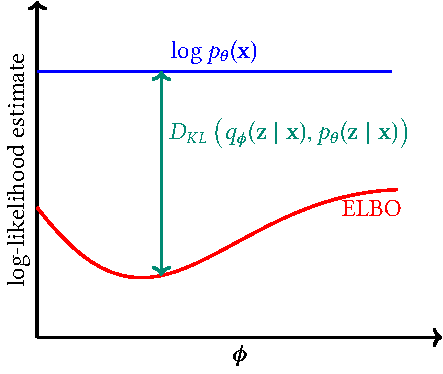
\includegraphics[width=0.8\linewidth]{../diagrams/elbo/elbo_diagram}
	\caption{ELBO is a lower bound of the log likelihood, the difference between the two is the KL divergence. The better the approximation of the posterior $q_{\boldsymbol{\phi}}(\mathbf{z}|\mathbf{x})$, the smaller is KL and consequently the closer is ELBO to $\log p_{\boldsymbol{\theta}}(\mathbf{x})$.}
	\label{fig:elbodiagram}
\end{figure}
\subsubsection{Gradient estimation}
\label{subsec:gradest}
In order to perform gradient descent on the ELBO objective, we need to be able to evaluate its gradients with respect to parameters $\boldsymbol{\theta}$ and $\boldsymbol{\phi}$. Taking the gradient w.r.t generative parameters $\boldsymbol{\theta}$ is straightforward, because we can change the order of the expectation operator and the gradient, leaving us with
\begin{equation}
	\begin{aligned} 
		\nabla_{\boldsymbol{\theta}} \mathcal{L}_{\boldsymbol{\theta}, \boldsymbol{\phi}}(\mathbf{x}) &=\nabla_{\boldsymbol{\theta}} 	\mathbb{E}_{q_{\boldsymbol{\phi}}(\mathbf{z} \mid \mathbf{x})}\left[\log p_{\boldsymbol{\theta}}(\mathbf{x}, \mathbf{z})-\log q_{\boldsymbol{\phi}}(\mathbf{z} | \mathbf{x})\right] \\  & \simeq \nabla_{\boldsymbol{\theta}}\left(\log p_{\boldsymbol{\theta}}(\mathbf{x}, \mathbf{z})-\log q_{\boldsymbol{\phi}}(\mathbf{z} | \mathbf{x})\right) \\ &=\nabla_{\boldsymbol{\theta}}\left(\log p_{\boldsymbol{\theta}}(\mathbf{x}, \mathbf{z})\right) ,
	\end{aligned}
\end{equation}
where $\simeq$ denotes an unbiased estimator. This reversing of the order of operations is not possible when taking gradients w.r.t variational parameters $\boldsymbol{\phi}$, because the expectation $\mathbb{E}_{q_{\boldsymbol{\phi}}(\mathbf{z} | \mathbf{x})}$ is performed w.r.t the approximate posterior $q_{\boldsymbol{\phi}}(\mathbf{z} | \mathbf{x})$. The gradient could be estimated with a vanilla Monte Carlo estimator, but it has very high variance and is not practical~\cite{kingma2013auto}. 

The problem of stochastic gradient estimation of an expectation of a function is a well studied problem that transcends machine learning and has a variety of applications~\cite{chriss1997black, schrittwieser2020mastering}. Different estimators differ in from and their properties, variance being one of the most important. In their review~\cite{mohamed2020monte} Mohamed et al. categorise MC gradient estimators into three categories
\begin{enumerate}
	\item \emph{Score-function estimator}: The score function is a logarithm of a probability distribution w.r.t to distributional parameters. It can be used as a gradient estimator
	\begin{equation}
		\begin{aligned}
		\nabla_{\boldsymbol{\theta}} \mathbb{E}_{p_{\boldsymbol{\theta}}(\mathbf{x})}[f(\mathbf{x})] &=  \nabla_{\boldsymbol{\theta}} \int p_{\boldsymbol{\theta}}(\mathbf{x}) f(\mathbf{x}) d \mathbf{x} \\
		&= \mathbb{E}_{p_{\boldsymbol{\theta}}(\mathbf{x})}\left[f(\mathbf{x}) \nabla_{\boldsymbol{\theta}} \log p_{\boldsymbol{\theta}}(\mathbf{x})\right].
		\end{aligned}
	\end{equation}
	The score-function estimator is compatible with any cost function, it requires that the measure $p_{\boldsymbol{\theta}}(\mathbf{x})$ is differentiable and easy to sample. Very importantly it is applicable to both discrete and continuous distribution, but has a drawback of having high variance.

	\item \emph{Pathwise estimator}: Continuous distributions can be sampled either directly by generating samples from the distribution $p_{\boldsymbol{\theta}}(\mathbf{x})$ or indirectly, by sampling from a simpler base distribution $p(\boldsymbol{\epsilon})$ and transforming the variate through a deterministic path $g_{\boldsymbol{\theta}}(\boldsymbol{\epsilon})$. Using this, it is possible to move the source of randomness in such a way that the objective is differentiable. In essence this approach pushes the parameters of the measure into the cost function which is then differentiated. The estimator is
	\begin{equation}
		\begin{aligned}
			\nabla_{\boldsymbol{\theta}} \mathbb{E}_{p_{\boldsymbol{\theta}}(\mathbf{x})}[f(\mathbf{x})] 
			 &=\nabla_{\boldsymbol{\theta}} \int p_{\boldsymbol{\theta}}(\mathbf{x}) f(\mathbf{x}) d \mathbf{x} \\
			 &= \nabla_{\boldsymbol{\theta}} \int p(\boldsymbol{\epsilon}) f(g_{\boldsymbol{\theta}}(\boldsymbol{\epsilon})) d \boldsymbol{\epsilon} \\
			 &= \mathbb{E}_{p(\boldsymbol{\epsilon})}\left[\nabla_{\boldsymbol{\theta}} f(g_{\boldsymbol{\theta}}(\boldsymbol{\epsilon}))\right].
		\end{aligned}
	\end{equation}
	\begin{figure}
		\subfloat[Original]{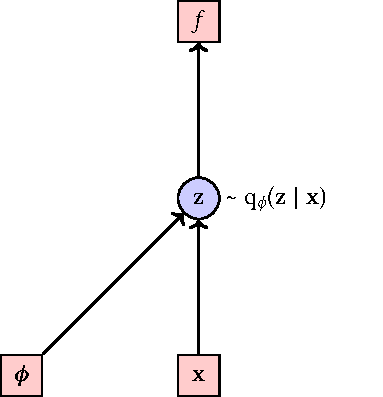
\includegraphics[height=3.8cm]{../diagrams/reparametrisation/reparam_diagram.pdf}}
		\subfloat[Reparametrized]{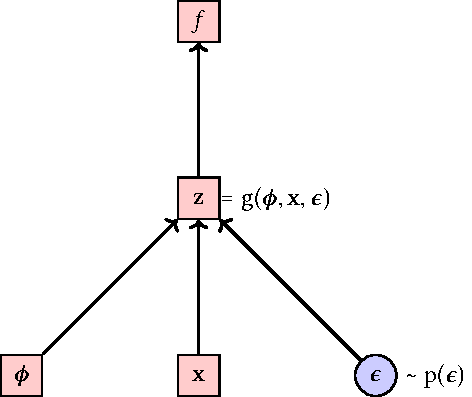
\includegraphics[height=3.8cm]{../diagrams/reparametrisation/reparam_diagram2.pdf}}
		\caption{The reparametrization trick, adapted from~\cite{kingma2017variational}. The stochasticity of the $\mathbf{z}$ node is pushed out into a separate input to the same node, resulting in deterministic gradients w.r.t $\boldsymbol{\phi}$ through the node.}
		\label{fig:reparam}
	\end{figure}
	This was the gradient estimator originally used in the VAE implementation~\cite{kingma2013auto} there named as the \emph{reparametrization trick}, see also Figure~\ref{fig:reparam}. In many cases the transformation paths are so simple they can be implemented in one line of code, referred to as \emph{one-liners}. The pathwise-estimator can only be used on differentiable cost functions, but is easy to implement and crucially has lower variance than the score-function estimator. 
	
	\item \emph{Measure-valued gradient estimator}, which exploits the properties of signed-measures is beyond the scope of this report.	
\end{enumerate}
	Unbiased gradient estimation makes training on the ELBO objective possible. During training the VAE learns a mapping between a complicated observed space of $\mathbf{x}$ and the latent space of $\mathbf{z}$, which is usually defined to be relatively simple. The \emph{decoder} network or the \emph{generative} part of the VAE $p_{\boldsymbol{\theta}}(\mathbf{x} | \mathbf{z})$ learns to map from the latent space to the data space, while the \emph{inference} or \emph{encoder} network $q_{\mathbf{\phi}}(\mathbf{z}|\mathbf{x})$ approximates the true posterior $p_{\mathbf{\theta}}(\mathbf{z}|\mathbf{x})$ of this process, see Figure~\ref{fig:vae_basic}. 

	\begin{figure}
		\centering
		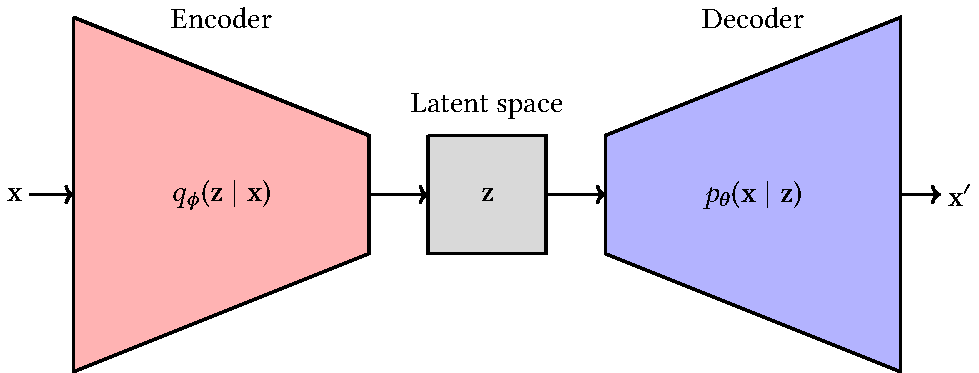
\includegraphics[width=\linewidth]{../diagrams/vae/vae_diagram.pdf}
		\caption{\label{fig:vae_basic} The variational autoencoder. }
	\end{figure}


\subsubsection{Variants and advances}
In the previous section we have described the basic variational autoencoder as proposed in the original paper~\cite{kingma2013auto}. But as with any new paradigm/approach in machine learning, the variational autoencoder was quickly extended in a variety of ways. A large line of work tries to address the issues that VAEs have with learning, this was prompted by the discovery that ELBO optimisation can get stuck in suboptimal equilibria~\cite{bowman2015generating}. Suggestions include annealing the latent cost $D_{K L}(q(\mathbf{z} | \mathbf{x}) \| p(\mathbf{z}))$ from $0$ to $1$~\cite{bowman2015generating}, or modifying the ELBO objective to ensure that a certain minimum number of bits is encoded in each latent variable~\cite{kingma2016improving}. The $\beta$-VAE~\cite{higgins2016beta} also modifies the ELBO objective by introducing the $\beta$ hyperparameter to balance the regularization and reconstruction terms. One thing that the $\beta$-VAE does particularly well is learn disentangled latent representations, which are latent representations where each component is sensitive to changes in one generative factor and is not much affected by others. Further work has been done in understanding how introducing the $\beta$ parameter leads to these representations~\cite{burgess2018understanding}. 

Alternative objectives to the evidence lower bound have also been proposed, instead of using the KL divergence one can use the chi-square divergence to arrive at an upper bound of the log likelihood (CUBO) and optimise that~\cite{dieng2016variational}. In addition to the objective of the VAE, any other component can be, and has been modified and studied. There has been work done on improving the variational posteriors by using conditional flow-based models~\cite{kingma2016improving, rezende2015variational}, implementing all sorts of architectures of the decoder, including convolutional neural networks, residual networks and recurrent neural networks~\cite{gregor2015draw}. 
% Other types of data and hierirchical + extension to semi supervised learning
Much in the same vein, variational autoencoders have been adapted for use with other data types than the original application to images. Among other uses, they have been used for text generation~\cite{semeniuta2017hybrid}, molecular graph generation~\cite{jin2018junction} and video compression~\cite{habibian2019video}. Variational autoencoders can also be used in tandem with a classifier in a procedure called semi-supervised learning~\cite{kingma2014semi}, allowing to learn from large datasets which have only partially been labeled. 

We have alluded in section~\ref{sec:DLVM} that VAEs can have hierarchical latent space structure, such models have very recently been implemented and show promising results. The Bidirectional-Inference Variational Autoencoder (BIVA)~\cite{maaloe2019biva} uses a skip-connected generative model and an inference network formed by a bidirectional stochastic inference path to learn a hierarchy of latent variables. Another hierarchical VAE is the Noveau-VAE (NVAE)~\cite{vahdat2020nvae} which uses depth-wise separable convolutions and batch normalization. Moreover, very deep VAE's~\cite{child2020very} can represent autoregressive models and beat them on likelihood benchmarks. 

Given the reliance of most variational autoencoders on the reparametrization trick, one of their main flaws is their inability to treat discrete latent variables. Current workarounds to this issue include using a continuous relaxation of the discrete latent variables~\cite{maddison2016discrelax}, or pairing each discrete latent variable with an auxiliary continuous one and performing the reparametrization trick on the marginal distributions~\cite{rolfe2016discrete}. Current state of the art is the vector quantised VAE (VQ-VAE) which uses vector quantisation for the latent space and learns the prior~\cite{DBLP:journals/corr/abs-1711-00937}.

% Problems
Nevertheless, there are some problems with VAEs that have not yet been fully addressed. Perhaps the most striking issue, one that pertains to all deep generative models not just VAEs, is the \emph{out-of-distribution problem}. Deep generative models have trouble distinguishing between a sample from the distribution they were trained on and another sample from a different distribution. This was discovered by Nalisnick et al.~\cite{nalisnick2018deep}, when they noticed that the models could not distinguish common objects (CIFAR-10) from house numbers (SVHN). The second problem is the \emph{posterior collapse}. Because of the variance of the stochastic gradient approximation the posterior approximation $q_{\boldsymbol{\phi}}(\mathbf{z} | \mathbf{x})$ may provide too weak of a signal 
\begin{equation}
	q_{\boldsymbol{\phi}}(\mathbf{z} | \mathbf{x}) \approx q_{\boldsymbol{\phi}}(\mathbf{z}),
\end{equation}
resulting in the decoder ignoring $\mathbf{z}$ samples from the posterior. Proposed solutions include skip connections~\cite{dieng2016variational} and aggressively optimising the inference model before performing each model update.~\cite{he2019lagging}. There is also the \emph{hole problem}~\cite{rezende2018taming}, which occurs when there are discrepancies between the prior $p(\mathbf{z})$ and the aggregate posterior $q_{\boldsymbol{\phi}}(\mathbf{z}) =  \frac{1}{N} \sum_{n} q_{\boldsymbol{\phi}}\left(\mathbf{z}| \mathbf{x}_{n}\right)$, where $\mathbf{x}_n$ is a training example. Sampling from these discrepancies or \emph{holes} provides poor latent variable samples which are then badly reconstructed by the generative network. Finally there is the \emph{balancing problem}, the issue of finding a good balance between the sampling quality and the reconstruction quality.

\section{Implementation of Variance loss}
The evidence lower bound (ELBO) pathwise gradient estimator (SGVB), described in section~\ref{subsec:gradest}, has found great success but is limited to models with continuous latent variables. It would be more convenient to have a loss function that would deal with both discrete and continuous latent variables within the same framework. Recent work by Richter et al.~\cite{richter2020vargrad} analysed a score-function gradient estimator for ELBO and showed that it can be obtained from a different divergence measure, which they termed the \emph{log-variance loss}
\begin{equation}
	\mathcal{L}_{\text{LV}}\left(q_{\boldsymbol{\phi}}(\mathbf{z}) \| p_{\boldsymbol{\theta}}(\mathbf{z} \mid \mathbf{x})\right)=\frac{1}{2} \underset{\mathbf{\mathbf{z}} \sim r(\mathbf{\mathbf{z}})}{\operatorname{\mathbb{V}ar}}\left[\log \left(\frac{q_{\boldsymbol{\phi}}(\mathbf{z})}{p_{\boldsymbol{\theta}}(\mathbf{z} \mid \mathbf{x})}\right)\right],
\end{equation}
where $r(\mathbf{z})$ is some arbitrary distribution. Moreover, they showed that the gradient of $\mathcal{L}_{\text{LV}}$ w.r.t $\boldsymbol{\phi}$ corresponds to that of the KL divergence if $r(\mathbf{\mathbf{z}}) = q_{\boldsymbol{\phi}}(\mathrm{z})$ and provided a gradient estimator of the log-variance, thus suggested an optimisation procedure that works for both discrete and continuous latent distributions. In this work we will proceed in a similar fashion but with a different loss function. Motivated by the fact that when the posterior $q(z | x) = p(z | x)$ is exact we have
\begin{equation}
	\frac{p(\mathbf{x} \mid \mathbf{z}) p(\mathbf{z})}{q(\mathbf{z} \mid \mathbf{x})}=p(\mathbf{x}).
\end{equation}
The variance of $p(\mathbf{x})$ with regards to samples drawn from an arbitrary probability distribution $r(\mathbf{z})$ which suggests the variance of the left hand side
\begin{equation}
	\mathcal{L}_{\boldsymbol{\phi}, \boldsymbol{\theta}}(\mathbf{x}) = \underset{\mathbf{z} \sim r(\mathbf{z})}{\operatorname{\mathbb{V}ar}}\left[\log \left(\frac{p_{\boldsymbol{\theta}}(\mathbf{x} \mid \mathbf{z}) p(\mathbf{z})}{q_{\boldsymbol{\phi}}(\mathbf{z} \mid \mathbf{x})}\right)\right]
\end{equation}
as an objective function. We can estimate the loss with sample variance using $S$ Monte Carlo samples
\begin{equation}
	\label{eq:varloss}
	\begin{aligned}
		\mathcal{L}_{\boldsymbol{\phi}, \boldsymbol{\theta}}(\mathbf{x}) \approx \frac{1}{(S-1)} &\sum_{s=1}^{S}\left(f_{\boldsymbol{\phi},\boldsymbol{\theta}}(\mathbf{z}^{(s)}, \mathbf{x})-\bar{f}_{\boldsymbol{\phi},\boldsymbol{\theta}}(\mathbf{x})\right)^{2}, \\
		\quad \mathbf{z}^{(s)} &\stackrel{\text { i.i.d. }}{\sim} r(\mathbf{z}),
	\end{aligned}
\end{equation}
where
\begin{equation}
	f_{\boldsymbol{\phi},\boldsymbol{\theta}} = \log \left(\frac{p_{\boldsymbol{\theta}}(\mathbf{x} \mid \mathbf{z}) p(\mathbf{z})}{q_{\boldsymbol{\phi}}(\mathbf{z} \mid \mathbf{x})}\right)
\end{equation}
and $f_{\boldsymbol{\phi},\boldsymbol{\theta}}$ is the average
\begin{equation}
	\bar{f}_{\boldsymbol{\phi},\boldsymbol{\theta}}(\mathbf{x})=\frac{1}{S} \sum_{s=1}^{S} f_{\boldsymbol{\phi},\boldsymbol{\theta}}\left(\mathbf{z}^{(s)},  \mathbf{x}\right).
\end{equation}
The gradient of expression~\eqref{eq:varloss} can be computed using automatic differentiation without any issue. The form of the gradient estimator of $\mathcal{L}_{\boldsymbol{\phi}, \boldsymbol{\theta}}(\mathbf{x})$ outlined above, is the same as the leave-one-out estimator described in~\cite{richter2020vargrad}, which means that it is an unbiased estimator of the gradient. The procedure of calculating the gradients for a given example $\mathbf{x}$ and parameters $\boldsymbol{\phi}, \boldsymbol{\theta}$ is given in Algorithm~\ref{alg:vargradEst}.
\begin{algorithm}[h]
	\SetAlgoLined
	\KwIn{Encoder parameters $\boldsymbol{\phi}$, decoder parameters $\boldsymbol{\theta}$, example $\mathbf{x}$}
	\KwResult{Gradients w.r.t $\boldsymbol{\phi}, \boldsymbol{\theta}$ of the objective function $1$}
		\For{s = 1, \ldots, S}{
		$\boldsymbol{z}^{(s)} \leftarrow \operatorname{sample}\left(q_{\boldsymbol{\phi}}(\cdot \mid \mathbf{x})\right)$ \\
		$\boldsymbol{z}^{(s)} \leftarrow \operatorname{ stop\_gradient }\left(\boldsymbol{z}^{(s)}\right)$ \\
		$f_{\boldsymbol{\phi}, \boldsymbol{\theta}}^{(s)} \leftarrow \log p_{\boldsymbol{\theta}}\left(\boldsymbol{x} | \boldsymbol{z}^{(s)}\right)p\left(\boldsymbol{z^{(s)}}\right) - \log q_{\phi}\left(z^{(s)}\right)$
	}
	$\widehat{\mathcal{L}} \leftarrow \text { Variance }\left(\left\{f_{\boldsymbol{\phi}, \boldsymbol{\theta}}^{(s)}\right\}_{s=1}^{S}\right)$ \\
	
	\Return $\operatorname{grad}\left(\widehat{\mathcal{L}}\right)$
	\caption{\label{alg:vargradEst}Gradients of $\mathcal{L}_{\boldsymbol{\boldsymbol{\phi}}, \boldsymbol{\theta}}(\mathbf{x})$}
\end{algorithm}
Importantly the samples $\mathbf{z}^{(s)}$, which will be for simplicity sampled from the model probability $\mathbf{z} \sim  q_{\boldsymbol{\phi}}(\mathbf{z} \mid \mathbf{x})$, must be detached from the computational graph so that backpropagation is possible. 

To test the applicability of the loss function we will test two variational autoencoders, one with continuous latent space and one with discrete latent space. The architecture of the neural networks that were used to parameterise the encoder and decoder will be discussed in section~\ref{sec:results}.

\subsection{Continuous latent space}
\label{subsec:continuous}
For the continuous case we will recreate the model from the original VAE paper~\cite{kingma2013auto}. The inference and generative models will both be parameterised by fully connected multilayer perceptrons. The approximate posterior $q_{\boldsymbol{\phi}}(\mathbf{z} \mid \mathbf{x})$ will be a multivariate Gaussian with a diagonal covariance matrix
\begin{equation}
	\label{eq:gaussian}
	\begin{aligned}
		q_{\boldsymbol{\phi}}(\mathbf{z} \mid \mathbf{x}) &=\mathcal{N}\left(\mathbf{z} ; \boldsymbol{\mu},  \operatorname{diag}\left(\sigma^{2}\right)\right) \\
		q_{\boldsymbol{\phi}}(\mathbf{z} \mid \mathbf{x}) & =\prod_{i} q_{\boldsymbol{\phi}}\left(z_{i} \mid \mathbf{x}\right)=\prod_{i} \mathcal{N}\left(z_{i} ; \mu_{i}, \sigma_{i}^{2}\right)
	\end{aligned}
\end{equation}
where
\begin{equation}
	(\boldsymbol{\mu}, \log \boldsymbol{\sigma})=\text { EncoderNeuralNet }_{\boldsymbol{\phi}}(\mathbf{x}).
\end{equation}
The choice of decoder depends on the type of data. For real-valued outputs the generative $p_{\boldsymbol{\theta}}(\mathbf{z} | \mathbf{x})$ model is again a Gaussian, with mean and variance parameterised by a neural network
\begin{equation}
	(\boldsymbol{\mu}, \log \boldsymbol{\sigma})=\text { DecoderNeuralNet }_{\boldsymbol{\theta}}(\mathbf{z}).
\end{equation}
Alternatively if the outputs are binary we use the Bernoulli distribution for the logarithm of $p_{\boldsymbol{\theta}}(\mathbf{x} | \mathbf{z})$
\begin{equation}
	\label{eq:bernoulli}
	\begin{aligned} 
		\log p_{\boldsymbol{\theta}}(\mathbf{x} \mid \mathbf{z}) 
		&=\sum_{j=1}^{D} \log p\left(x_{j} \mid \mathbf{z}\right) \\ 
		&=\sum_{j=1}^{D} \log \operatorname{Bernoulli}\left(x_{j} ; y_{j}\right) \\ 
		&=\sum_{j=1}^{D} x_{j} \log y_{j}+\left(1-x_{j}\right) \log \left(1-y_{j}\right).
	\end{aligned}
\end{equation}
Where $D$ is the dimension of $\mathbf{x}$ and $\mathbf{y}$ is the output of a sigmoid activation in the last layer of the NN
\begin{equation}
	\mathbf{y}=f_{\sigma}\left(\text{DecoderNeuralNet}_{\boldsymbol{\theta}}(\mathbf{z})\right).
\end{equation}
The prior $p(\mathbf{z})$ will be a unit isotropic Gaussian in either case $p(\mathbf{z})=\mathcal{N}(\mathbf{z} ; \mathbf{0}, \mathbf{I})$. 

\subsection{Discrete latent space}
\label{subsec:discrete}


\section{Experiments}
\label{sec:results}
\subsection{Continuous latent space}
We compare the performance of the latent variable model described in section~\ref{subsec:continuous} and compare the efficiency of different gradient estimators/objectives.

\subsubsection{Fashion MNIST}
\subsubsection{CELEBa}

\subsection{Discrete latent space}
\subsubsection{Binarized MNIST}
\subsubsection{Binarized Omniglot}

\section{Conclusion}





\bibliographystyle{elsarticle-num}
\bibliography{WA1-references.bib}

\end{document}

%%
%% End of file `elsarticle-template-num.tex'.
